% Author Vahid Partovi Nia
% Copyright Huawei Technologies
% Network Mind Team



\documentclass[12pt]{beamer}

\usetheme{Hannover}
\setbeamercolor{section in sidebar shaded}{fg=black}

\usecolortheme{beaver}
\beamertemplatenavigationsymbolsempty

%  \usebeamertemplate{navigation symbols}\hfill
%  \insertframenumber{}/\inserttotalframenumber}
  

\useoutertheme{sidebar}
\pgfdeclareimage[width=2.5\baselineskip]{institut-logo}{fig/mcgill_logo}
\setbeamertemplate{footline}
{\raisebox{-2ex}{\pgfuseimage{institut-logo}}
%  \hfill
\hspace{5cm}
  \usebeamertemplate{navigation symbols}
  \insertframenumber{}/\inserttotalframenumber
  \hspace{3.8cm}
YCBS255
}
%\setbeamertemplate{sidebar right}{}
  
\setbeamercolor{block title}{fg=darkred}
\setbeamercolor{local structure}{fg=darkred}

\setbeamercolor{palette sidebar secondary}{fg=darkgray, bg=white}



\usefonttheme{professionalfonts} % using non standard fonts for beamer


\makeatletter
\beamer@nav@subsectionstyle{hide/hide/hide}
\makeatother

\titlegraphic{
\includegraphics[width=2cm]{fig/mcgill_logo}}




\usepackage{listings}
\usepackage{xcolor}
\def \y {\mathbf y}
\def \z {\mathbf z}
\def \Z {\mathbf Z}
\def \X {\mathbf X}
\def \A {\mathbf A}
\def \t {^\top}
\def \inv {^ {-1}}
\def \x {\mathbf x}
\def \bbeta {\boldsymbol \beta}
\def \eeps {\boldsymbol \varepsilon}
\def \TV {\mathrm{TV}}
\def \Radio {\mathrm{Radio}}
\def \Newspaper {\mathrm{Newspaper}}
\def \Sales {\mathrm{Sales}}
\def \Balance {\mathrm{Balance}}
\def \Default {\mathrm{Default}}
\def \M {\mathcal{M}}

\def \r {\mathbf{r}}
\def \e {\mathbf{e}}

\def \RSS {\mathrm{RSS}}

\def \E {\mathrm{E}}
\def \P {\mathbf{P}}

\def \V {\mathrm{V}}
\def \cor {\mathrm{cor}}

\def \SSigma {\boldsymbol{\Sigma}}
\def \LLambda {\boldsymbol{\Lambda}}
\def \pphi {\boldsymbol{\phi}}
\def \PPhi {\boldsymbol{\Phi}}
\def \mmu {\boldsymbol{\mu}}
\def \ttheta {\boldsymbol{\theta}}


\definecolor{capri}{rgb}{0.0, 0.75, 1.0}
\definecolor{darkcyan}{rgb}{0.0, 0.55, 0.55}
\definecolor{deepfuchsia}{rgb}{0.76, 0.33, 0.76}
\begin{document}
% no title and no author on sidebar
\title[]{Dimension Reduction}   
\author[]{Vahid Partovi Nia} 
\institute{Lecture 06}
\date{}


\makeatletter
  \begin{frame}[plain]
    \hspace*{-\beamer@leftsidebar}%
    \advance\textwidth by \beamer@leftsidebar\relax
    \beamer@leftsidebar=\z@
    \begin{minipage}{\textwidth}\par%
      \maketitle
    \end{minipage}
  \end{frame}
  \makeatother



\frame{\frametitle{Outline}\tableofcontents} 

\setbeamertemplate{sidebar left}[sidebar theme]

\section{Projection}
\begin{frame}[fragile]\frametitle{Projection}
Suppose $$\x = (x_1, \ldots, x_p)\t.$$ 
Dimensions reductuin is about projection of $\x$ onto a new space  $$\z=(z_1,\ldots,z_m)\t$$ with a new dimension $m<p$.
\end{frame}

\begin{frame}[fragile]\frametitle{Linear projection}
If projection is linear  
\begin{eqnarray*}
z_1 &=& \sum_{j=1}^p \phi_{j1} x_j \\
z_2 &=&  \sum_{j=1}^p \phi_{j2} x_j \\
\vdots\\
z_m &=& \sum_{j=m}^p \phi_{jm} x_j \\
\end{eqnarray*}
How to find good coefficients $\phi_{jm}$
\end{frame}

\begin{frame}[fragile]\frametitle{What linear projection mean?}
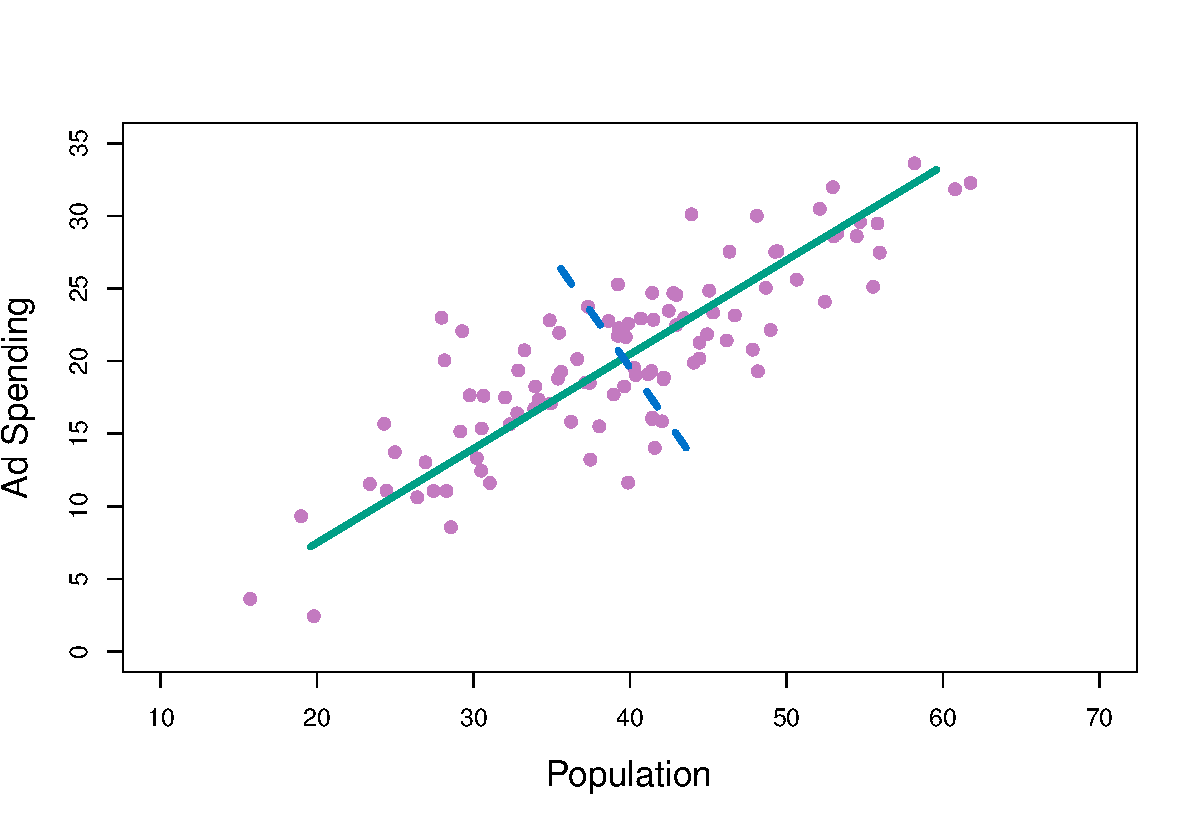
\includegraphics[width=0.9\textwidth]{fig/6-14}
\end{frame}

\frame{\frametitle{Data projection}
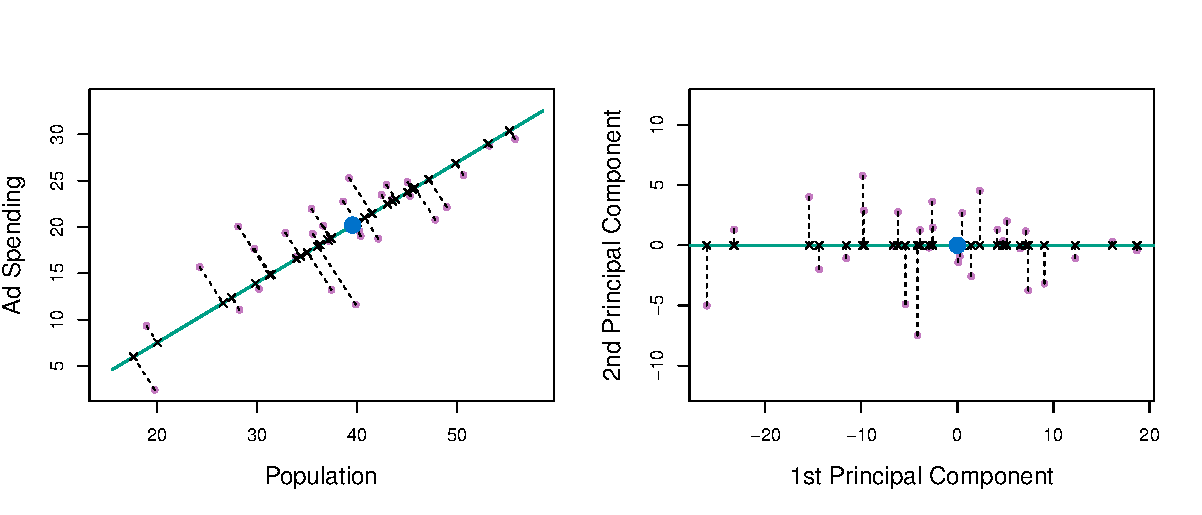
\includegraphics[width=\textwidth]{fig/6-15}
}

\frame{\frametitle{How to find projection coefficients}
Remember for a univariate random variable $x$ 
\begin{eqnarray*}
\E(\phi x) &=& \phi \E(x)\\
\V(\phi x) &=& \phi^2 \V(x)
\end{eqnarray*}
For a multivariate $\x, \E(\x) = \mmu, \V(\x)= \SSigma$
\begin{eqnarray*}
\E(\pphi\t \x) &=& \pphi\t \E(\x) = \phi \mmu \\
\V(\pphi\t \x) &=& \pphi\t \V(\x) \pphi = \pphi\t \SSigma \pphi
\end{eqnarray*}
}

\section{Principal Components}

\frame{\frametitle{Principal components}
\begin{itemize}
\item  Find $\pphi_1$ so that $\V(\z_1) = \V(\pphi_1\t\x)$ is maximized.
\item Find $\pphi_2$ so that $\pphi_2 \perp \pphi_1$ and $\V(\z_2) = \V(\pphi_2\t\x)$ is maximized.
\item Find $\pphi_3$ so that $\pphi_3 \perp \pphi_1,\pphi_2$ and $\V(\z_3) = \V(\pphi_3\t\x)$ is maximized.
 $$\vdots$$
\item Find $\pphi_m$ so that $\pphi_3 \perp \pphi_1,\ldots,\pphi_{m-1}$ and $\V(\z_m) = \V(\pphi_m\t\x)$ is maximized.
\end{itemize}
}

\frame{\frametitle{Find the first projection}
Suppose $\V(\x)=\SSigma$ has an eigen value decomposition $\SSigma = \P \LLambda \P\t$\\
\begin{itemize}
\item $\LLambda = \mathrm{diag}(\lambda_i)$
\item $\P\t\P= \P\P\t = \mathbf I$ 
\end{itemize}
It is easy to show that $\lambda_{\max} = \max {\V(\pphi\t \x)\over \pphi\t \pphi} $ and the maximizer is $\hat\pphi = \e_{\max}$
}


\begin{frame}[fragile]\frametitle{PCA}
\tiny	
\begin{lstlisting}
import pandas as pd
path='data/'
filename = path+'Auto.csv'
auto = pd.read_csv(filename, 
	na_values=['?'], na_filter=True)
auto = auto.dropna()
\end{lstlisting} 
\pause
\begin{lstlisting}
X = auto[['cylinders', 'displacement', 
	'horsepower', 'weight', 
	'acceleration']]

y = auto['mpg']
\end{lstlisting} 
\pause
\begin{lstlisting}
from sklearn.decomposition import PCA
pca = PCA(n_components=2)
pca.fit(X.values)
Z = pca.transform(X)
\end{lstlisting} 
\pause
\begin{lstlisting}
import matplotlib.pyplot as plt
%matplotlib inline
plt.scatter(Z[:,0], Z[:,1]);
\end{lstlisting} 
\end{frame}


\begin{frame}[fragile]\frametitle{Standardized PCA}
\tiny	
\begin{lstlisting}
from sklearn.preprocessing import scale
X_std = scale(X.values)
pca_std = PCA(n_components=2)
pca_std.fit(X_std)
Z_std = pca_std.transform(X_std)
plt.scatter(Z_std[:,0], Z_std[:,1]);
\end{lstlisting} 
\end{frame}

\frame{\frametitle{Principal component regression}
After finding the coefficients, projecting $x$ to the new dimension provides $\Z_{n\times m}$.\\
Now one can use the projected dimensions to predict a response variable $y$.
$$ \y = \X\bbeta +\eeps $$
\begin{eqnarray*}
\Z_{n \times m} &=& \X_{n\times p} \PPhi_{p\times m} \\
\y &=& \Z\ttheta +\eeps
\end{eqnarray*} 
This is called principal component regression, $\Z$  involves no collinearity!
}

\section{Principal Component Regression}
\begin{frame}[fragile]\frametitle{PCR}
\tiny	
\begin{lstlisting}
from sklearn.linear_model import LinearRegression
lr = LinearRegression()
X_simple = X[['horsepower']]
lr.fit(X_simple,y)
lr.score(X_simple, y)
\end{lstlisting} 
\pause
\begin{lstlisting}
pcr = LinearRegression()
Z_simple = Z[:,0].reshape(-1,1)
pcr.fit(Z_simple, y)
pcr.score(Z_simple,y)
\end{lstlisting} 
\end{frame}

\section{Partial Least Squares}

\frame{\frametitle{Partial least squares}
If regression with $y$ is the reason of projection, it makes sense to project $x$ to orthogonal axes, while correlation to $y$ is accounted for.
\begin{itemize}
\item PCA: $\max {\V(\pphi\t \x)} $
\item PLS: $\max {\V(\pphi\t \x)\cor^2(\pphi\x , y)} $
\end{itemize}
}


\begin{frame}[fragile]\frametitle{}
\tiny	
\begin{lstlisting}
from sklearn.cross_decomposition import PLSRegression
pls = PLSRegression(n_components=2)
pls.fit(X, y)
W = pls.transform(X)
plt.scatter(W[:,0], W[:,1]);
\end{lstlisting} 
\pause
\begin{lstlisting}
pls.score(X,y)
\end{lstlisting} 
\end{frame}

\section{Zip Code}



\begin{frame}[fragile]\frametitle{}
\tiny	
\begin{lstlisting}
path='data/'
filename = path+'ziptrain.csv'
import numpy as np
zipdata = np.loadtxt(filename)

zipdata.shape
\end{lstlisting} 

\begin{lstlisting}
plt.imshow(-zipdata[0, 1:].reshape(16,16), "gray");
\end{lstlisting} 

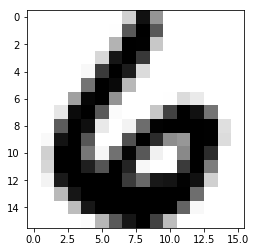
\includegraphics[width=0.3\textwidth]{fig/zip6} \pause
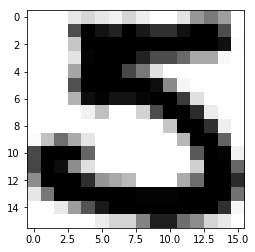
\includegraphics[width=0.3\textwidth]{fig/zip5}\\
\pause

\begin{lstlisting}
zipdata3=zipdata[zipdata[:, 0] == 3]
zipdata8=zipdata[zipdata[:, 0] == 8]
zipdata38 = np.vstack([zipdata3, zipdata8])

pca = PCA(n_components=2)
pca.fit(zipdata38[:, 1:])
Z = pca.transform(zipdata38[:,1:])
plt.scatter(Z[:,0], Z[:,1], c= zipdata38[:,0], alpha=0.3);
\end{lstlisting} 
\end{frame}

\frame{\frametitle{}
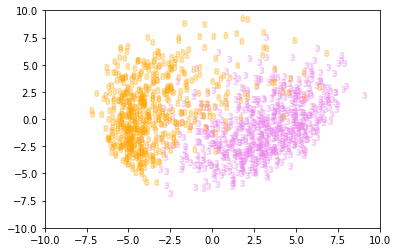
\includegraphics[width=\textwidth]{fig/zip38}
}


%\frame{\frametitle{}
%\includegraphics[width=0.5\textwidth]{fig/}
%}

%\frame{\frametitle{}
%\includegraphics[width=0.5\textwidth]{fig/}
%}

%\frame{\frametitle{}
%\includegraphics[width=0.5\textwidth]{fig/}
%}
%

%\frame{\frametitle{}
%\includegraphics[width=0.5\textwidth]{fig/}
%}
%
%
%

\end{document}
